\documentclass[10pt]{beamer} 
\usetheme{cwc} 

\usepackage{amsmath,amssymb}
\usepackage{graphicx,acronym,setspace,epstopdf}
\usepackage[ruled]{algorithm2e}
\usepackage{subeqnarray,multirow,cite,array,color,mathtools}

\acrodef{MSE}{mean squared error}
\acrodef{BC}{broadcast channel}
\acrodef{MC}{multi-cell}
\acrodef{BS}{base station}
\acrodef{MIMO}{multiple-input multiple-output}
\acrodef{SISO}{single-input single-output}
\acrodef{MU}{multi-user}
\acrodef{MU-MIMO}{\acl{MU} \acl{MIMO}}
\acrodef{OFDM}{orthogonal frequency division multiplexing}
\acrodef{WSRM}{weighted sum rate maximization}
\acrodef{QoS}{quality of service}
\acrodef{SCA}{successive convex approximation}
\acrodef{SNR}{signal-to-noise ratio}
\acrodef{MMSE}{minimum \acl{MSE}}
\acrodef{SIR}{signal-to-interference ratio}
\acrodef{SINR}{signal-to-interference-plus-noise ratio}
\acrodef{Q-WSRM}{queue \acl{WSRM}}
\acrodef{QM}{queue minimizing}
\acrodef{SRA}{spatial resource allocation}
\acrodef{JSFRA}{joint space-frequency resource allocation}
\acrodef{WMMSE}{weighted \acl{MMSE}}
\acrodef{KKT}{Karush-Kuhn-Tucker}
\acrodef{GP}{geometric programming}
\acrodef{SOC}{second-order cone}
\acrodef{BCDM}{block coordinate descent method}

\newcommand{\mbf}[1]{\mathbf{#1}}
\newcommand{\me}[1]{\( #1 \)}
\newcommand{\mc}[1]{\mathcal{#1}}
\newcommand{\fall}{\forall}
\newcommand{\set}[1]{\left \lbrace #1 \right \rbrace }
\newcommand{\mvec}[2]{\mathbf{#1}_{#2}}
\newcommand{\ith}[1]{{#1}^\mathrm{th}}
\newcommand{\pr}[1]{{#1}^\prime}
\newcommand{\mbfa}[1]{{\boldsymbol{#1}}}
\newcommand{\herm}{\mathrm{H}}
\newcommand{\sset}[1]{\left [ #1 \right ]}
\newcommand{\rfrac}[2]{{}^{#1}/{}_{#2}}
\newcommand{\eqspace}{\IEEEeqnarraynumspace}
\newcommand{\enoise}{\widetilde{N}_0}
\newcommand{\eqsub}{\IEEEyessubnumber}
\newcommand{\review}[1]{{\textcolor[rgb]{0 0 0.6}{#1}}}
\newcommand{\trace}{\mathrm{tr}}
\newcommand{\tran}{\mathrm{T}}
\newcommand{\R}[1]{\label{#1}\linelabel{#1}}
\newcommand{\lr}[1]{page~\pageref{#1}, line~\lineref{#1}}
\newcommand{\eqn}[1]{\(#1\)}
\newcommand{\mx}{\mbf{m}}
\newcommand{\my}{\mbf{w}}
\newcommand{\mz}{\mbfa{\gamma}}
\newcommand{\mxb}{{{\mbf{m}}}}
\newcommand{\myb}{{{\mbf{w}}}}
\newcommand{\iterate}[2]{{#1}^{(#2)}}
\newcommand{\iter}[3]{{#1}_{#2}^{(#3)}}
\newcommand{\ma}{\mbf{x}}
\acrodef{MSE}{mean squared error}
\acrodef{IBC}{interference broadcast channel}
\acrodef{MC}{multi-cell}
\acrodef{BS}{base station}
\acrodef{MIMO}{multiple-input multiple-output}
\acrodef{SISO}{single-input single-output}
\acrodef{MU}{multiple users}
\acrodef{OFDM}{orthogonal frequency division multiplexing}
\acrodef{WSRM}{weighted sum rate maximization}
\acrodef{QoS}{quality of service}
\acrodef{SCA}{successive convex approximation}
\acrodef{SNR}{signal-to-noise ratio}
\acrodef{MMSE}{minimum \acl{MSE}}
\acrodef{SIR}{signal-to-interference ratio}
\acrodef{SINR}{signal-to-interference-plus-noise ratio}
\acrodef{Q-WSRM}{queue \acl{WSRM}}
\acrodef{QM}{queue minimizing}
\acrodef{SRA}{spatial resource allocation}
\acrodef{JSFRA}{joint space-frequency resource allocation}
\acrodef{WMMSE}{weighted \acl{MMSE}}
\acrodef{KKT}{Karush-Kuhn-Tucker}
\acrodef{GP}{geometric programming}
\acrodef{SOC}{second-order cone}
%\acrodef{BCDM}{block coordinate descent method}
\acrodef{ADMM}{alternating directions method of multipliers}
\acrodef{PD}{primal decomposition}
\acrodef{DD}{dual decomposition}
\acrodef{FFR}{fractional frequency reuse}
\acrodef{DC}{difference of convex}
\acrodef{Q-WSRME}{\ac{Q-WSRM} extended}
\acrodef{TDD}{time division duplexing}
\acrodef{CSI}{channel state information}
\acrodef{AO}{alternating optimization}
\acrodef{OTA}{over-the-air}
\acrodef{PL}{path loss}
\acrodef{TDM}{time division multiplexing}
\acrodef{UC}{uncoordinated}

\graphicspath{{./../Figures/}{./../Figures/Linux/}{./../Figures/Review/}}
\DeclareGraphicsExtensions{.eps}

\epstopdfsetup{update,prepend,prefersuffix=false,suffix=}
\DeclareGraphicsRule{.eps}{pdf}{.pdf}{`epstopdf #1}
\pdfcompresslevel=9

\title{Traffic Aware Precoder Design for Space Frequency Resource Allocation}
\author{{Ganesh Venkatraman, Antti T\"{o}lli, Le-Nam Tran and Markku Juntti} \\ \scriptsize{Email: \{gvenkatr, antti.tolli, le.nam.tran, markku.juntti\}@ee.oulu.fi}}

\begin{document}

\AtBeginSection{\frame{\sectionpage}}

\begin{frame}
    \titlepage
\end{frame}

\begin{frame}{Outline}
    \tableofcontents
\end{frame}

\section{Introduction}

\begin{frame}{Introduction and Motivation}
\begin{itemize}
\item Complex algorithms are adopted to maximize the throughput to satisfy the data requirements of the higher layers
\item Available wireless resources are to be utilized efficiently to minimize the backlogged packets 
\item Spatial and Frequency resources are exploited to empty the packets waiting at the \acsp{BS}
\item In this work, we discuss the precoder design for the \acl{MU} \acs{MIMO}-\acs{OFDM} setup to minimize the number of queued packets 
\end{itemize}
\end{frame}

\section{System Model \& Problem Formulation}

\begin{frame}{Symbols used}
\begin{itemize}
\item \acs{OFDM} system with \me{N} sub-channels and \me{N_B} \acp{BS}, each equipped with \me{N_T} transmit antennas
\item Let \me{K} be the total number of users with \me{N_R} antennas
\item Let \me{\mc{B}} and \me{\mc{U}} denote the set of coordinating \acp{BS} and users in the system
\item The set of users belonging to \acs{BS} \me{b} is denoted by \me{\mc{U}_b \in \mc{U}}
\item Let \me{b_k \in \mathcal{B}} denotes the \ac{BS} serving the user \me{k}
\item Let \me{L} be the total available spatial streams for a user \me{k}, given by \me{\min (N_T,N_R)}
\end{itemize}
\end{frame}

\begin{frame}{System Model}
\begin{itemize}
\item The \me{\ith{l}} spatial signal received on sub-channel \me{n} of user \me{k} is given by
\begin{multline}\label{eqn-1}
\hat{d}_{l,k,n} = \mvec{w}{l,k,n}^\herm \mvec{H}{b_k,k,n} \,\mvec{m}{l,k,n} d_{l,k,n} + \mvec{w}{l,k,n}^\herm \mvec{n}{l,k,n} \\ 
+ \mvec{w}{l,k,n}^\herm \sum_{i \in \mc{U} \backslash \set{k}} \mvec{H}{b_i,k,n} \sum_{j = 1}^L \mvec{m}{j,i,n}d_{j,i,n}
\end{multline}
\item where \me{\mvec{m}{l,k,n}} and \me{\mvec{w}{l,k,n}} are transmit and receive beamformers corresponding to the \me{\ith{l}} spatial stream on the \me{\ith{n}} sub-channel of user \me{k}
\end{itemize}
\end{frame}

\begin{frame}{System Model}
\begin{itemize}
\item \me{\mvec{H}{b_k,k,n} \in \mathbb{C}^{N_R \times N_T}} denotes the channel between \ac{BS} \me{b_k} and user \me{k}
\item \me{d_{l,k,n}} and \me{{n}_{l,k,n}} correspond to data symbol and equivalent noise on \me{\ith{l}} spatial stream of user \me{k}
\item Using the above notations, the \acs{SINR} seen by the \me{\ith{l}} spatial stream on the \me{\ith{n}} sub-channel for user \me{k} is given by
\end{itemize}
\begin{equation}\label{eq:SINR}
\gamma_{l,k,n} = \dfrac{\left |\mvec{w}{l,k,n}^\herm \, \mvec{H}{b_k,k,n} \, \mvec{m}{l,k,n} \right |^2}{\enoise + \sum_{(j,i) \neq (l,k)} |\mvec{w}{l,k,n}^\herm \mvec{H}{b_i,k,n} \mvec{m}{j,i,n} |^2}
\end{equation}
\begin{itemize}
\item where \eqn{\enoise = \|\mvec{w}{l,k,n}^\herm \mvec{n}{l,k,n} \|^2 }
\end{itemize}
\end{frame}

\begin{frame}{Queueing Model}
\begin{itemize}
\item Each user is associated with backlogged packets of size \me{Q_k} packets.
\item Queued packets \me{Q_k} of each user follows dynamic equation at the \me{\ith{i}} instant as
\begin{equation}
Q_k(i+1) = \Big [ Q_k(i) - t_k(i) \Big ]^+ + \lambda_k(i)
\label{eqn-2a}
\end{equation}
\item where \me{t_k = \sum_{n = 1}^N \, \sum_{l = 1}^L \, t_{l,k,n}} denotes the total number of transmitted packets corresponding to user \me{k} in the previous \me{\ith{i}} instant
\item \me{\lambda_k} represents the fresh arrivals of user \me{k} at \ac{BS} \me{b_k}
\end{itemize}
\end{frame}

\begin{frame}{Problem Formulation}
\begin{itemize}
\item Objective is to transmit the queued packets waiting at \acsp{BS} to corresponding users in the system.
\item The available spatial and frequency resources are to be efficiently utilized to minimize the queued packets
\item In order to achieve this, precoders are to be designed with certain objective that involves the backlogged packets as well
\item Precoders can perform scheduling of users by providing zero powers to exclude from the resource elements
\end{itemize}
\end{frame}

\section{Centralized Solutions}

\subsection{Existing \acs{Q-WSRM} Formulation}

\begin{frame}{Queue-Weighted Sum Rate Maximization (\acs{Q-WSRM})}
\begin{itemize}
\item \acs{Q-WSRM} formulation is the result of minimizing the conditional Lyapunov drift \footnote{Neely, Michael J. "Stochastic network optimization with application to communication and queueing systems." Synthesis Lectures on Communication Networks 3.1 (2010): 1-211.}
\item \acs{Q-WSRM} formulation is also called as back pressure algorithm, since it acts greedily in minimizing the backlogged packets at each instant
\[ \underset{t_{l,k,n}}{\text{minimize}} \quad \sum_{k \in \mc{U}} \left \lbrace Q_k(i)^2 - Q_k(i-1)^2 \right \rbrace, \]
\item where \me{Q_k} follows the dynamic Queue expression in \eqref{eqn-2a} and \me{t_k = \sum_{n = 1}^N \, \sum_{l=1}^L \, t_{l,k,n}}
\end{itemize}
\end{frame}

\begin{frame}{Queue-Weighted Sum Rate Maximization (\acs{Q-WSRM})}
\begin{itemize}
\item Upon solving the Lyapunov drift expression, we obtain the \acs{Q-WSRM} formulation as
\end{itemize}
\begin{subequations}
\begin{align}
 \underset{t_{l,k,n}}{\text{maximize}} & \qquad \sum_{k \in \mc{U}} \; Q_k \left ( \alert{\sum_{n=1}^N} \, \sum_{l = 1}^L  t_{l,k,n} \right ) \\
& \qquad {\color{blue} \alert{\sum_{n=1}^N} \, \sum_{l = 1}^L  t_{l,k,n}  \leq \alert{Q_k} \; / \; Q_{k,n}}
\end{align}
\end{subequations}
\begin{itemize}
\item Performs better in cell-edge scenarios
\item Complexity can be reduced if precoders are designed for each sub-channel independently
\end{itemize}
\end{frame}

\begin{frame}{Queue-Weighted Sum Rate Maximization (\acs{Q-WSRM})}
	\begin{itemize}
		\item Complexity can be reduced if precoders are designed for each sub-channel independently
		\item Coupling across sub-channels is obtained by the queues, which are updated after evaluating the rate from previously chosen sub-channels as
	\end{itemize}
	\begin{equation*}
	Q_{k,n} = \max{\Big \lbrace Q_k - \sum_{j = 1}^{n-1} \, \sum_{l = 1}^{L} \, t_{l,k,j} ,0 \Big \rbrace }, \; \forall \; k \in \mathcal{U}
	\end{equation*}
\end{frame}

\subsection{\acs{JSFRA} Formulation (\acs{SINR} Relaxation)}

\begin{frame}{\acs{JSFRA} Formulation (\acs{SINR} Relaxation)}
\begin{itemize}
\item Precoders are designed by a centralized controller, which are then used by all \acp{BS} in \me{\mc{B}}
\item The objective used to design transmit precoders is 
\[ {\color{blue} v_k = \left | Q_k - \sum_{n = 1}^N \sum_{l = 1}^{L} t_{l,k,n} \right |^q } \]
\item To generalize the objective, we use \me{\tilde{v}_k \triangleq a_k \, v_k}, where \me{a_k} is arbitrary weights used control the priorities
\item Exponent \me{q} plays different role based on the value it assumes
	\begin{itemize}
	\item \me{\ell_{q=1}} results in greedy allocation
	\item \me{\ell_{q=2}} ideal for the delay or buffer size limited scenarios
	\item \me{\ell_{q=\infty}} provides fair resource allocation in each transmission instant
	\end{itemize}
\end{itemize}
\end{frame}

\begin{frame}{\acs{JSFRA} Formulation (\acs{SINR} Relaxation)}
\begin{itemize}
\item Now, the precoder design problem is given as
\end{itemize}
\begin{subequations} \label{eqn-6}
\begin{align}
\underset{{t_{l,k,n},\mvec{M}{k,n},\mvec{W}{k,n}}}{\text{minimize}} & \hspace{0.25em} && \| \tilde{\mbf{v}} \|_q \label{eqn-obj} \\
\text{subject to} & \hspace{0.25em} && t_{l,k,n}\leq \log_2(1 + \gamma_{l,k,n}) \\
& \hspace{0.25em} && \alert{\gamma_{l,k,n} \leq \dfrac{\left |\mvec{w}{l,k,n}^H \, \mvec{H}{b_k,k,n} \, \mvec{m}{l,k,n} \right |}{\beta_{l,k,n}}^2\triangleq f(\tilde{\mbf{u}}_{l,k,n})},\label{eqn-6.2}\\
& \hspace{0.25em} && \beta_{l,k,n}  \geq  \enoise + \sum_{(j,i) \neq (l,k)} |\mvec{w}{l,k,n}^H \mvec{H}{b_i,k,n} \mvec{m}{j,i,n} |^2, \label{eqn-6.3} \\
& \hspace{0.25em} && \sum_{n = 1}^N \sum_{k \in \mathcal{U}_b} \text{tr} \, (\mvec{M}{k,n} \mvec{M}{k,n}^H) \leq P_{{\max}}, \fall b
\end{align}
\end{subequations}
\begin{itemize}
\item where \me{\tilde{\mbf{u}}_{l,k,n}  \triangleq \{\mvec{w}{l,k,n}^H, \mvec{H}{b_k,k,n}, \mvec{m}{l,k,n},\beta_{l,k,n}\}}
\end{itemize}
\end{frame}

\begin{frame}{\acs{JSFRA} Formulation (\acs{SINR} Relaxation)}
\begin{itemize}
\item To maximize the received \acs{SINR}, \me{\mvec{w}{l,k,n}} are modeled with the \acs{MMSE} receivers
\item The \acs{JSFRA} formulation in \eqref{eqn-6} is nonconvex due to the constraint defined by \eqref{eqn-6.2} as
\me{\alert{\gamma_{l,k,n} \leq \dfrac{\left |\mvec{w}{l,k,n}^H \, \mvec{H}{b_k,k,n} \, \mvec{m}{l,k,n} \right |}{\beta_{l,k,n}}^2}}
\item In order to solve the problem in \eqref{eqn-6}, we use \ac{SCA} approach for the constraint defined by \eqref{eqn-6.2}
\item Let, \me{f(\tilde{\mbf{u}}_{l,k,n})=(p_{l,k,n}^2 + q_{l,k,n}^2)/\beta_{l,k,n}}, where
\end{itemize}
\begin{subeqnarray}
p_{l,k,n} &\triangleq& \Re \set{{\mvec{w}{l,k,n}^H \mvec{H}{b_k,k,n} \mvec{m}{l,k,n}}}, \\
q_{l,k,n} &\triangleq& \Im \set{{\mvec{w}{l,k,n}^H \mvec{H}{b_k,k,n} \mvec{m}{l,k,n}}}
\end{subeqnarray}
\end{frame}

\begin{frame}{\acs{JSFRA} Formulation (\acs{SINR} Relaxation)}
\begin{itemize}
\item Now, the first order Taylor approximation is used for the function \me{f(\tilde{\mbf{u}}_{l,k,n})} around an arbitrary point \me{\tilde{\mbf{u}}_{l,k,n}^{(i-1)}}
\item With this approximation, the problem in \eqref{eqn-6} can be solved using the well known solvers for the optimal precoders and \me{\tilde{\mbf{u}}_{l,k,n}}
\item Once the precoders \me{\mvec{m}{l,k,n}} are evaluated, \me{\mvec{w}{l,k,n}} are updated using the \acs{MMSE} receivers
\item The local point \me{\tilde{\mbf{u}}_{l,k,n}^{(i-1)}} is updated with the current optimal point \me{\tilde{\mbf{u}}_{l,k,n}^{(i)}}
\item With the updated precoders and \me{\tilde{\mbf{u}}_{l,k,n}^{(i)}}, optimization is carried out in an iterative manner until convergence
\end{itemize}
\end{frame}

\subsection{\acs{JSFRA} Formulation (\acs{MSE} Reformulation)}

\begin{frame}{\acs{JSFRA} Formulation (\acs{MSE} Reformulation)}
	\begin{itemize}
		\item In this approach, we utilize the relation between the \acs{MSE} and the \acs{SINR} as \me{\color{blue} \epsilon_{l,k,n} = (1 + \gamma_{l,k,n})^{-1}}
		\item Equivalence is valid only when the receivers are designed with the \ac{MSE} objective, \textit{i.e.}, using \acs{MMSE} receivers
	\end{itemize}
	\begin{multline} \label{mse-error}
	\mathbb{E} \big [ ( d_{l,k,n} - \hat{d}_{l,k,n} )^2 \big ] = \left | 1 - \mvec{w}{l,k,n}^\herm \mvec{H}{b_k,k,n} \mvec{m}{l,k,n} \right |^2 \\
		+ \sum_{{(j,i) \neq (l,k)}} \left | \mvec{w}{l,k,n}^\herm \mvec{H}{b_i,k,n} \mvec{m}{j,i,n} \right |^2 + \enoise = \epsilon_{l,k,n}
	\end{multline}
\end{frame}

\begin{frame}{\acs{JSFRA} Formulation (\acs{MSE} Reformulation)}
	\begin{itemize}
		\item Using the above reformulation, we can formulate the \acs{JSFRA} problem as
	\end{itemize}
	\begin{subeqnarray} \label{eqn-mse-1}
		\underset{\substack{t_{l,k,n},\mvec{m}{l,k,n},\\ \epsilon_{l,k,n},\mvec{w}{l,k,n}}} {\text{minimize}} & \quad & \|  \tilde{\mbf{v}}^{\prime}  \|_q \label{eqn-mse-1.1} \\
		\text{subject to} &\quad & \alert{t_{l,k,n} \leq -\log_2(\epsilon_{l,k,n})}  \slabel{eqn-mse-1.2} \\
		& \quad & {\color{blue} \sum_{{(j,i) \neq (l,k)}} \left | \mvec{w}{l,k,n}^\herm \mvec{H}{b_i,k,n} \mvec{m}{j,i,n} \right |^2 + \enoise} \nonumber \\	
		&\quad & {\color{blue} \qquad {} + \left | 1 - \mvec{w}{l,k,n}^\herm \mvec{H}{b_k,k,n} \mvec{m}{l,k,n} \right |^2 \leq \epsilon_{l,k,n}} \slabel{eqn-mse-1.3} \\
		&\quad & \sum_{n = 1}^N \sum_{k \in \mathcal{U}_b} \sum_{l=1}^L \trace \, (\mvec{m}{l,k,n} \mvec{m}{l,k,n}^\herm) \leq P_{{\max}} \; \fall b.  \slabel{eqn-mse-1.4}
	\end{subeqnarray}
\end{frame}

\begin{frame}{\acs{JSFRA} Formulation (\acs{MSE} Reformulation)}
	\begin{itemize}
		\item The nonconvex constraint in \eqref{eqn-mse-1.2} is approximated by a sequence of convex constraints
		\item It is achieved by using \ac{SCA} technique as earlier
		\item The iterative procedure is performed until convergence or for suitable number of iterations
		\item \alert{The above reformulation works only with the \acs{MMSE} receiver}
	\end{itemize}
\end{frame}

\section{Distributed Solutions}

\subsection{Primal \& \acs{ADMM} based decompositions}

\begin{frame}{Distributed Methods}
	\begin{itemize}
		\item When the system size is small, centralized approach is viable if the channel remains constant for multiple transmission slots
		\item However, the overhead involved in the centralized design scales up significantly as the network size grows
		\item Distributed schemes based on primal decomposition or \acs{ADMM} can be used to reduce the signaling requirements
		\item The overhead involved in the design of precoders are only scalar interference variables
		\item Only the convex approximated subproblem in each \acs{SCA} step is performed via distributed approaches
	\end{itemize}
\end{frame}

\begin{frame}{Primal Decomposition Method}
	\begin{itemize}
		\item Precoder design is performed by a master-slave approach
		\item Interference created to the neighboring \ac{BS} users are bounded by a scalar variable
		\item The interference thresholds are determined by the master problem, which is performed at each \ac{BS} with the signaling exchange
	\end{itemize}
	\begin{equation} \label{inter_exp}
	\zeta_{l,k,n,b} \geq \sum_{i \in \mc{U}_b} \sum_{j = 1}^L |\mvec{w}{l,k,n}^\herm \mvec{H}{b,k,n} \mvec{m}{j,i,n} |^2 \; \forall b \in \bar{\mc{B}}_{b_k}.
	\end{equation}
	\begin{itemize}
		\item Each \ac{BS} subproblem includes \eqref{inter_exp} as an additional interference constraint in the respective optimization problem
	\end{itemize}
\end{frame}

\begin{frame}{ADMM based Decomposition Method}
	\begin{itemize}
		\item The \ac{ADMM} is superior to other distributed schemes in terms of the convergence speed
		\item The \ac{ADMM} includes an additional quadratic term in the objective as \me{\color{blue} \| \mbfa{\zeta}_b - \mbfa{\zeta}^{(j)}_b \|^2}, where \eqn{\mbfa{\zeta}^{(j)}_b} is global consensus variable
		\item Unlike primal decomposition method, \eqn{\zeta_{l,k,n,b}} in \eqref{inter_exp} is treated as an optimization variable in \ac{ADMM}
		\item The consensus variables are updated as
	\end{itemize}
	\begin{equation}
	\mbfa{\zeta}_{b_k}(b)^{(j+1)} = \mbfa{\zeta}_{b}(b_k)^{(j+1)} = \frac{\mbfa{\zeta}_{b}(b_k) + \mbfa{\zeta}_{b_k}(b)}{2}.
	\label{if-sg-update}
	\end{equation}
	\begin{itemize}
		\item where \eqn{\mbfa{\zeta}_{b_k}(b)} denotes the entries corresponding to \ac{BS} \eqn{b} in \ac{BS} \eqn{b_k}
	\end{itemize}
\end{frame}

\subsection{KKT based Distributed Solution}

\begin{frame}{KKT based Distributed Solution}
	\begin{itemize}
		\item The decentralization methods considered so far involve considerable signaling exchanges via backhaul
		\item However, when the users are equipped with multiple receive antennas, the overhead requirement is significantly large
		\item Since the signaling requirements are large, the iterative algorithm should design efficient precoders in few number of iterations to reduce the backlogged packets
		\item In order to achieve that, we design an iterative procedure based on solving the \ac{KKT} equations for the \acs{JSFRA} problem via \acs{MSE} reformulation
		\item Unlike the earlier schemes, we perform the group update of all the involved optimization variables to speed up the convergence of precoder design
	\end{itemize}
\end{frame}


\begin{frame}{KKT based Distributed Solution}
	\renewcommand{\arraystretch}{0.8} \scriptsize
\begin{subeqnarray} \label{kkt-mse-4}
	\mvec{m}{l,k,n}^{(i)} &=& \Big ( \sum_{x \in \mc{U}} \sum_{y=1}^L \alpha_{y,x,n}^{(i-1)} \mvec{H}{b_k,x,n}^\herm \mvec{w}{y,x,n}^{(i-1)} \mvec{w}{y,x,n}^{\herm \, {(i-1)}} \mvec{H}{b_k,x,n} + \delta_b \mbf{I}_{N_T} \Big )^{-1} \alpha^{(i-1)}_{l,k,n} \mvec{H}{b_k,k,n}^\herm \mvec{w}{l,k,n}^{(i-1)} \nonumber \\
	\mvec{w}{l,k,n}^{(i)} &=& \Big ( \sum_{x\in\mc{U}}\sum_{y=1}^L \mvec{H}{b_x,k,n} \mvec{m}{y,x,n}^{(i)} \mvec{m}{y,x,n}^{\herm \, (i)} \mvec{H}{b_{x},k,n}^\herm + N_0 \mathbf{I}_{N_R} \Big ) ^{-1} \; \mvec{H}{b_k,k,n} \; \mvec{m}{l,k,n}^{(i)} \label{kkt-mse-4.6}\\
	\epsilon_{l,k,n}^{(i)} &=& \left | 1 - \mvec{w}{l,k,n}^{\herm \, (i)} \mvec{H}{b_k,k,n} \mvec{m}{l,k,n}^{(i)} \right |^2 + \sum_{{(x,y) \neq (l,k)}} \left | \mvec{w}{l,k,n}^{\mathrm{H} \, (i)} \mvec{H}{b_y,k,n} \mvec{m}{x,y,n}^{(i)} \right |^2 + \enoise \label{kkt-mse-4.4} \\
	t_{l,k,n}^{(i)} &=&  -\log_2(\epsilon_{l,k,n}^{(i-1)}) - \frac{\left ( \epsilon_{l,k,n}^{(i)} - \epsilon_{l,k,n}^{(i-1)} \right ) }{\log(2) \, \epsilon_{l,k,n}^{(i-1)}} \label{kkt-mse-4.5} \\
	\sigma_{l,k,n}^{(i)} &=& \left [\tfrac{a_k \, q}{\log(2)}  \, \Big (Q_k - \sum_{n = 1}^N \sum_{l=1}^L t_{l,k,n}^{(i)} \Big )^{(q-1)}\right ]^+  \label{kkt-mse-4.2} \\
	\alpha^{(i)}_{l,k,n} &=& \alpha^{(i-1)}_{l,k,n} + \rho^{(i)} \left ( \tfrac{\sigma_{l,k,n}^{(i)}}{\epsilon_{l,k,n}^{(i)}} - \alpha^{(i-1)}_{l,k,n} \right ) \label{kkt-mse-4.1}
\end{subeqnarray}
\end{frame}

\section{Simulation Results}

\subsection{SISO Example}

\begin{frame}{\acs{SISO} Example}
\begin{itemize}
\item Let us consider a simple example with \me{N_T = N_R = 1}, \me{N=3} sub-channels, and \me{K = 3} users
\end{itemize}
\begin{table} \scriptsize
	\caption{Sub-channel-wise listing of channel gains and rate allocations}
	\begin{tabular}{|*{13}{c|}}
		\hline
		$Q_k$ & \multicolumn{3}{c|}{\eqn{\mvec{H}{b_k,k}}} & \multicolumn{3}{c|}{(A)} & \multicolumn{3}{c|}{(B)} & \multicolumn{3}{c|}{(C)} \\
		\cline{2-13}
		& \me{1} & \me{2} & \me{3} & \me{1} & \me{2} & \me{3} & \me{1} & \me{2} & \me{3} & \me{1} & \me{2} & \me{3} \\
		\hline
		\me{4} & \me{1.71} &  \me{0.53}  &  \me{0.56} & \me{0} &  \me{0}  &  \me{0} & \me{4.0} &  \me{0}  &  \me{0} & \me{0} &  \me{0}  &  \me{0} \\
		\me{8} & \me{0.39} &  \me{1.41}  &  \me{1.03} & \me{0} &  \me{4.88}  &  \me{3.11} & \me{0} &  \me{5.49}  &  \me{0} & \me{0} &  \me{4.39}  &  \me{3.53} \\
		\me{4} & \me{2.34} &  \me{1.26}  &  \me{2.32} & \me{4.0} &  \me{0}  &  \me{0} & \me{0} &  \me{0}  &  \me{4.0} & \me{5.81} &  \me{0}  &  \me{0} \\
		\hline
		\multicolumn{4}{|c|}{Remaining packets (\me{\chi})} & \multicolumn{3}{c|}{\me{3.92} bits} & \multicolumn{3}{c|}{\me{2.51} bits} & \multicolumn{3}{c|}{\me{5.89} bits} \\
		\hline
	\end{tabular}
	\label{tbl-1}
\end{table}
\begin{itemize}
\item \me{\zeta = \sum_{k = 1}^K \left [ \, Q_k - t_k \,\right ]^+}
\item \me{\zeta = 5.89} bits for \acs{Q-WSRM} (C), \me{\zeta = 3.92} bits for \acs{Q-WSRME} scheme (A) and, \me{\zeta = 2.51} bits for \acs{JSFRA} scheme (B)
\end{itemize}
\end{frame}

\subsection{MIMO Examples}

\subsubsection{Centralized Solutions}

\begin{frame}{Performance Comparison with Number of Residual Packets}
\begin{figure}
	\centering
	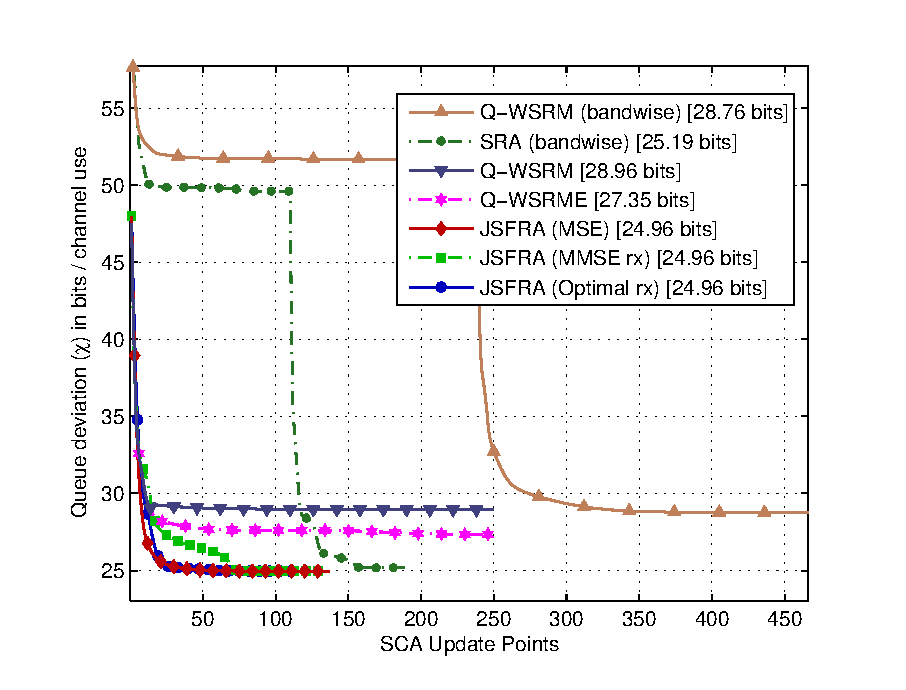
\includegraphics[width=0.75\textwidth]{fig-2-5}
	\caption{System Model - \me{\lbrace N,N_B,K,N_T,N_R \rbrace = \lbrace 2,3,9,4,2\rbrace}}
\end{figure}
\end{frame}

\subsubsection{Distributed Solutions}

\begin{frame}{Performance Comparison with Number of Residual Packets}
	\begin{figure}
		\centering
		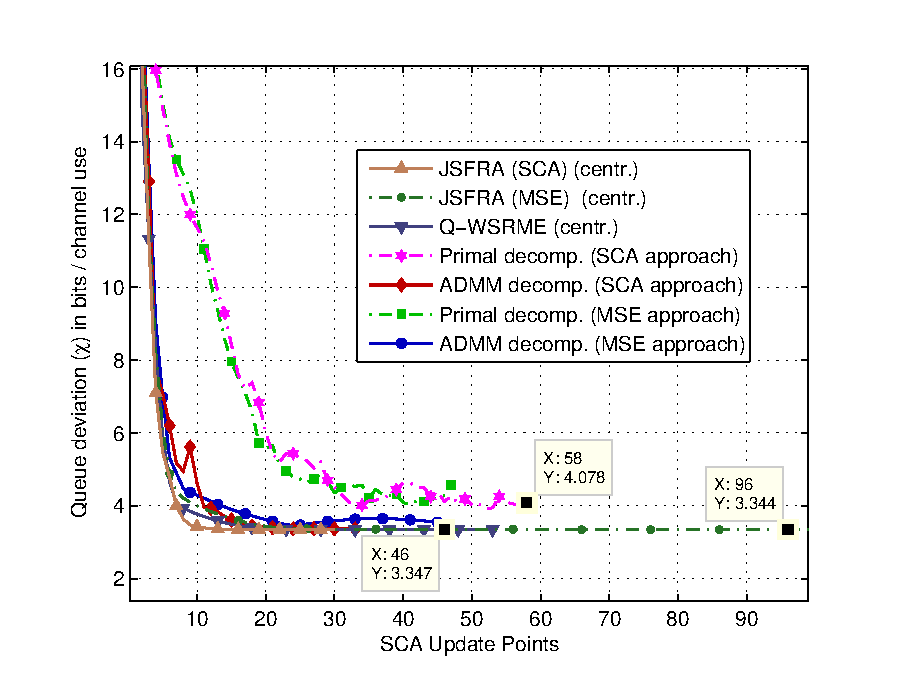
\includegraphics[width=0.75\textwidth]{fig-3-2}
		\caption{System Model - \me{\lbrace N,N_B,K,N_T,N_R \rbrace = \lbrace 3,2,8,4,1 \rbrace}}
	\end{figure}
\end{frame}

\subsubsection{Effect of varying \eqn{\ell_q} norms}

\begin{frame}{Effect on Residual Packets with different \eqn{\ell_q} norms}
	\begin{table}
		\centering
		\caption{Number of backlogged bits associated with each user for a system \me{\lbrace N,N_B,K,N_R \rbrace = \lbrace 5,2,8,1 \rbrace}.}
		\renewcommand{\arraystretch}{1.25} \scriptsize
		\begin{tabular}{|c|*{8}{c}|c|}
			\hline
			\multirow{2}{*}{\me{q}} & \multicolumn{8}{c|}{user indices} & \multirow{2}{*}{\me{\chi}} \\
			\cline{2-9}
			& 1 & 2 & 3 & 4 & 5 & 6 & 7 & 8 & \\
			\hline
			\hline
			\me{1} & 15.0 & 3.95 & 5.26 & 8.95 & 7.0 & 11.9 & 12.0 & 9.7 & 25.15 \\
			\me{2} & 11.2 & 3.9 & 10.76 & 10.65 & 10.27 & 9.68 & 8.77 & 5.9 & 27.77 \\
			\me{\infty} & 11.4 & 4.4 & 10.4 & 10.4 & 10.4 & 8.4 &  8.4 &  6.4 & 28.68 \\
			\hline
			\me{Q_k}  & 15.0 &  8.0 &  14.0 & 14.0 &  14.0 & 12.0 & 12.0 & 10.0  \\
			\cline{1-9}
		\end{tabular}
		\label{tbl-3}
	\end{table}	
\end{frame}

\subsubsection{KKT Based Approach}

\begin{frame}{Performance Comparison with Number of Residual Packets}
	\begin{figure}
		\centering
		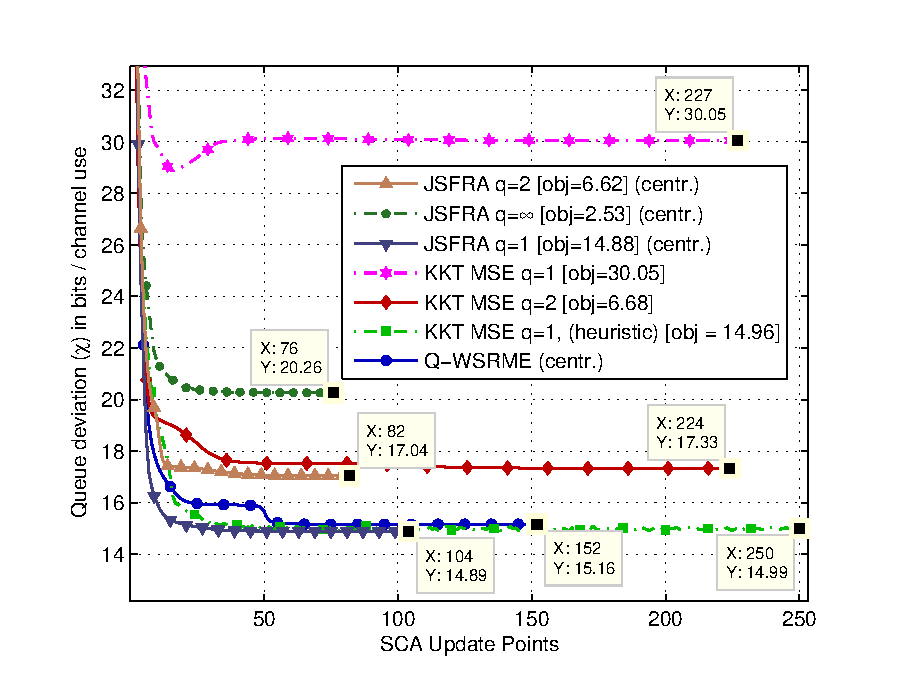
\includegraphics[width=0.75\textwidth]{fig-9-3}
		\caption{System Model - \me{\lbrace N,N_B,K,N_T,N_R \rbrace = \lbrace 5,2,8,4,1 \rbrace}}
	\end{figure}
\end{frame}

\subsection{Time Correlated Fading Performance}

\begin{frame}{Average Residual Packets after each Transmission Slot}
	\begin{figure}
		\centering
		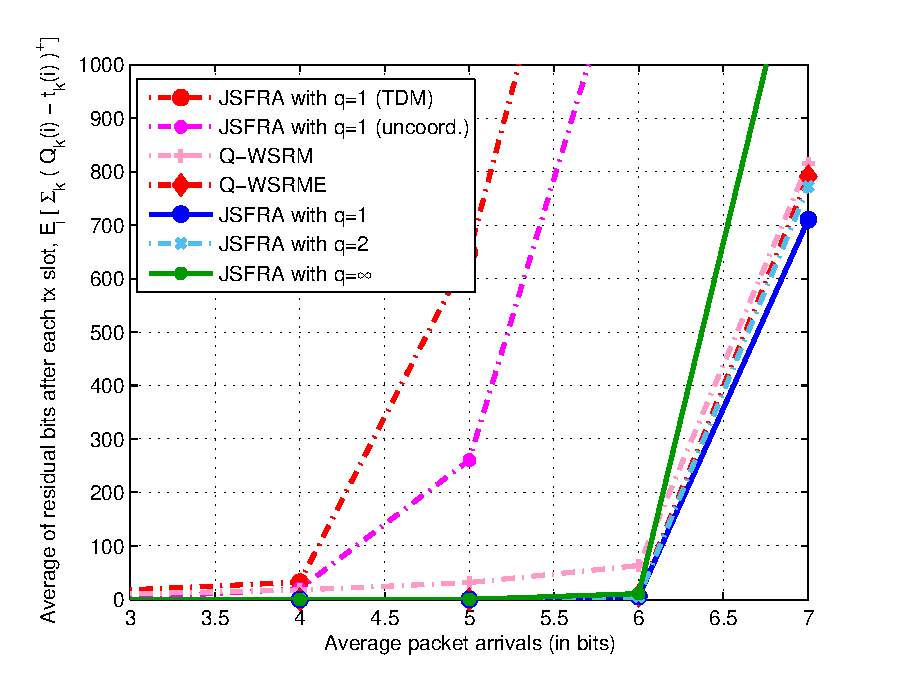
\includegraphics[width=0.75\textwidth]{average_queue_over_time-3}
		\caption{System Model - \me{\lbrace N,N_B,K,N_R \rbrace = \lbrace 3,2,8,1 \rbrace} after \eqn{250} transmissions}
	\end{figure}
\end{frame}

\section{Conclusions}

\begin{frame}{Conclusions}
\begin{itemize}
\item We discussed the problem of wireless resource allocation to minimize backlogged packets in an efficient way
\item The proposed approach uses \ac{SCA} method by using linear approximation for the nonconvex constraint
\item We also addressed different distributed methods for the precoder design across each \acsp{BS} with minimal information exchange
\item An iterative algorithm for the \acs{JSFRA} scheme using \acs{MSE} reformulation is also studied
\end{itemize}
\end{frame}


\begin{frame}
\begin{center}
{\color{blue}\Huge{Questions !}}
\end{center}
\end{frame}

\end{document}
